
\section{Einstellen eines PID-Reglers} 

\subsection{Vorgehensweisen zum Einstellen eines Reglers}

\begin{minipage}[c]{0.43\columnwidth}
    Regler-Entwuft ist \textbf{iterativer Prozess!}
    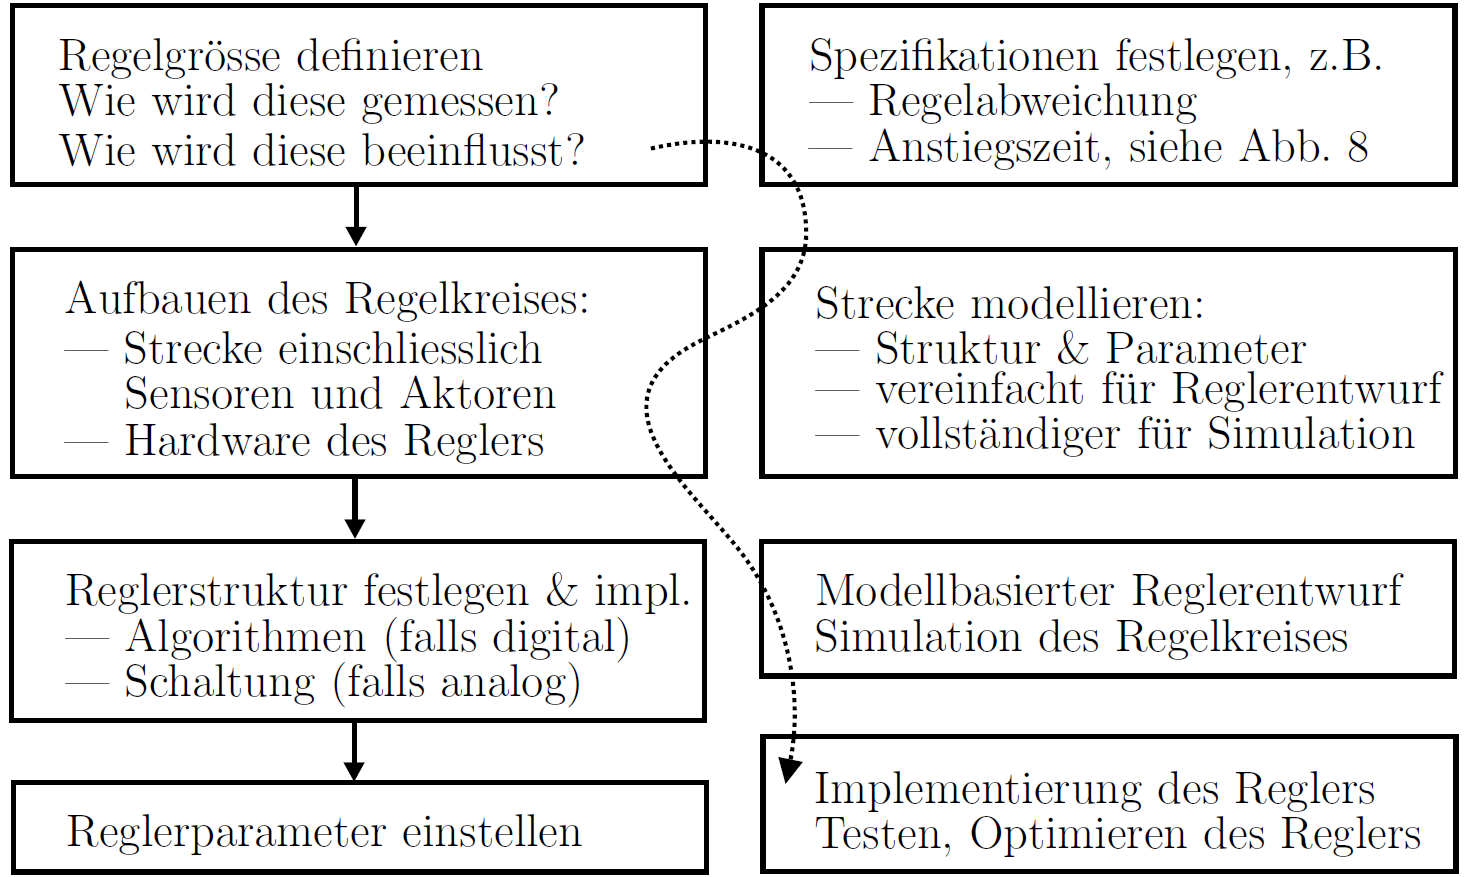
\includegraphics[width=\columnwidth]{images/reglerentwurf_moegliche_schritte.png}
\end{minipage}
\hfill
\begin{minipage}[c]{0.56\columnwidth}
    \begin{outline}
        \1 Experimente an realen Stecken
            \2 Sprungantworten und Frequenzantworten
        \1 Empirische Einstellregeln
            \2 Ziegler/Nichols, Chien/Hrones/Reswick, ...
        \1 Experimente an einem Modell der Strecke
            \2 Simulationen (viele!)
            \2 Sättigung, Rauschen, Unsicherheiten, ...
        \1 Analytischer Entwuft mit einem Modell
            \2 Pol-/Nullstellenkürzung, ...
    \end{outline}
\end{minipage}


\subsubsection{Reale Stecke vs. Modell}

\begin{outline}
    \1 Für einfache Strecken kann komplett auf Modell verzichtet werden
        \2 Zweipunkteregler, P-Regler für Wasserstand
        \2 Trial-and-Error
    \1 Modelle bieten Vorteile
        \2 Strecke ist nicht zugänglich
            \3 Prototyp; nur in kleinen Stückzahlen verfügbar; steht beim Kunden, ...
        \2 Tests dauern lange wegen grosser Zeitkonstante (\textrightarrow\ langes Messen)
        \2 Strecke ist gefährlich (z.B. Atomreaktor)
        \2 Messungen sind schlecht reproduzierbar
\end{outline}


\subsubsection{Analytischer Entwuft vs. Experiment}

\begin{minipage}[t]{0.48\columnwidth}
    \begin{outline}
        \1 Analytischer Entwuft und Analyse mit LZI-Modell
            \2 Sprungantworten (Führungsverhalten, Störverhalten)
            \2 Ortskurven / Bode-Diagramme
            \2 Verstärkungs- und Phasenreserve
            \2 Einfluss von Rauschen
        \1 Simulation mit Nicht-LZI (nichtlinear, zeitvariant)
            \2 Test der Funktionsfähigkeit mit 'genauerem' Modell
            \2 Unterscheidung von Betriebsfällen (Umschaltvorgänge)
                \3 Einschalten, Dauerbetrieb, Fehlerfälle
                \3 Zustandsautomaten
            \2 Wiederholbarkeit gewährleistet
    \end{outline}
\end{minipage}
\hfill
\begin{minipage}[t]{0.48\columnwidth}
    \begin{outline}
        \1 Regler-Tuning mit Experimenten
            \2 Man sieht, spürt und hört den Einfluss des Reglers sofort
                \3 z.B. Vibrationen
            \2 Messungen zur Beurteilung des Reglers (Robustheit) sinnd oft aufwändig
            \2 Experimente können lange dauern und sind oft auch schlecht reproduzierbar
            \2 Man kann sich keien Fehler erlauben!
                \3 Sicherer Betrieb muss gewährleistet sein
    \end{outline}
\end{minipage}


\subsubsection{Kriterien zur Beurteilung des Reglers}

\begin{minipage}[t]{0.48\columnwidth}
    \begin{outline}
        \1 Analytische Modelle
            \2 Pol-Lagen (Zeitkonstanten)
            \2 Frequenzgang (Nyquist, Bode)
            \2 Stabilitätsreserven
            \2 Sprungantworten 
                \3 Überhöhungen, Zeitkonstante
            \2 Gütemasse
    \end{outline}
\end{minipage}
\hfill
\begin{minipage}[t]{0.48\columnwidth}
    \begin{outline}
        \1 Experimente
            \2 Sprungantworten
                \3 Überhöhungen, Zeitkonstante
            \2 Berechnen von Gütemassen 
                \3 z.B. Integration Fehlerquadrat $e(t)^2$ und Stellgrössen $u(t)^2$
            \2 Geräusch-Entwicklung
            \2 Vibrationen
    \end{outline}
\end{minipage}


\subsection{Pol-Nullstellenkürzung}{164}

Hierbei handelt es sich um eine \textbf{analytische} Einstellmetode \textrightarrow\ LZI-Modell der Strecke muss vorliegen!
Der Regler wird dann so entworfen, dass er die \textbf{invertierte Stecke} enthält.
\begin{align*}
    G_R(s) &= \frac{K_R}{s} G_s^{-1}(s) \\
    G_0(s) &= G_R(s) \cdot G_S(s) \frac{K_R}{s} G_s^{-1}(s) \cdot G_S(s) = \frac{K_R}{s} \text{ \textrightarrow\ Integrator} \\
    G_f(s) &= \frac{G_0(s)}{1 + G_0(s)} = \frac{1}{\frac{1}{K_R} s + 1} \text{ \textrightarrow\ PT}_1 \text{-System} 
\end{align*}

\textbf{Hinweis:} Wähle als Reglerstruktur die Standardform (Variante 2) \textrightarrow\ siehe Abschnitt~\ref{PID-Regler Standardform}
\vspace{0.2cm}
Für die Übertragungsfunktionen gelten die folgenden Bezeichnungen:

\begin{minipage}[t]{0.48\columnwidth}
    \begin{tabular}{ll}
    $G_R(s)$    & UTF Regler \\
    $G_S(s)$    & UTF Stecke
\end{tabular}
\end{minipage}
\hfill
\begin{minipage}[t]{0.48\columnwidth}
    \begin{tabular}{ll}
        $G_0(s)$    & UTF offener Regelkreis \\
        $G_f(s)$    & UTF geschlossener Regelkreis  
    \end{tabular}
\end{minipage}


\subsubsection{Eigenschaften der Pol-Nullstellenkürzung}

\begin{outline}
    \1 \textbf{Pol-Nullstellenkürzung darf nur in der linken komplexen Halbebene durchgeführt werden!}
    % \1 Offener Regelkreis $G_0(s)$ wird zu einem Integrator \textrightarrow\ Optimalfall!
    % \1 Geschlossener Regelkreis $G_f(s)$ wird zu einem $\text{PT}_1$-System \textrightarrow\ Optimalfall!
    \1 Das Konzept funktioniert nicht immer
        \2 Inverse $G_s^{-1}(s)$ kann sehr sensitiv auf Modellparameter sein \\
            \textrightarrow\ braucht sehr genaues Modell
        \2 Instabile Stecken
        \2 Stecken mit Verzögerungen bzw. Totzeiten (\textrightarrow\ Regler wird akausal)
\end{outline}


\subsection{Empirische Einstellregeln}

\textbf{Idee:} Anhand weniger Messungen versucht man, über die Stecke genug Informationen zu gewinnen, um einen Regler entwerfen
zu können.


\subsubsection{Einstellung via Schrittantwort}{164-166}

\textbf{Idee:} Eine Stecke wird mit einem Eingangssignal $u(t) = A \cdot \varepsilon(t)$ angeregt und ihre 
Schrittantwort $y(t)$ wird gemessen. An diese gemessene Schrittantwort $y(t)$ wird ein \textbf{$\text{PT}_1$-System mit Totzeit}
'gefittet'. Die daraus entstehenden Parameter werden für die Regler-Dimensionierung verwendet.
$$ \text{PT}_1 \text{-System mit Totzeit} \quad G_0(s) = \frac{K_s}{s \cdot T_g + 1} e^{- s T_u} $$

\begin{minipage}[c]{0.45\columnwidth}
    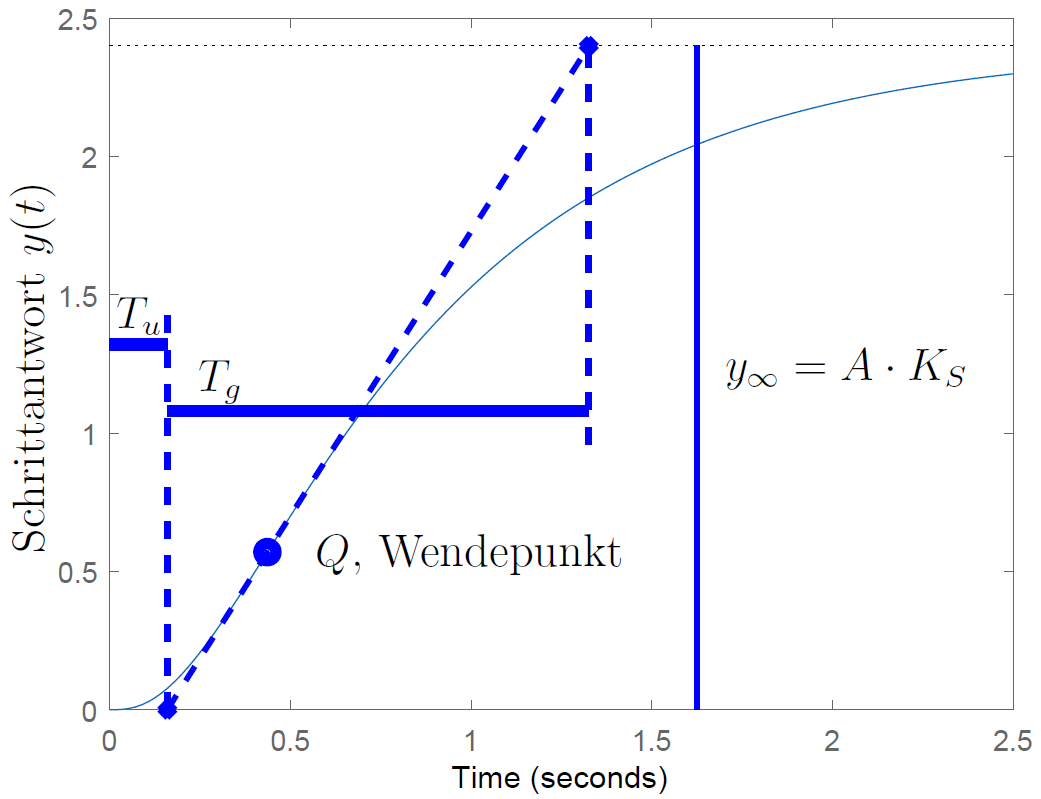
\includegraphics[width=\columnwidth]{images/pid_regler_empirisch_einstellen.png}
\end{minipage}
\hfill
\begin{minipage}[c]{0.52\columnwidth}
    \begin{center}
        \textbf{\myul{Vorgehen $\text{PT}_1$ fitten / Parameter bestimmen}}
    \end{center}

    \begin{outline}
        \1 Tangente an Wendepunkt $Q$ einzeichnen
        \1 Parameter $T_u$, $T_g$ und $K_s$ gemäss Grafik bestimmen
            \2 $K_s$: Verstärkung
            \2 $T_u$: Verzugszeit
            \2 $T_g$: Ausgleichszeit
        \1 Konstanten für Tabellen bestimmen
            \2 $\mu = \frac{T_g}{T_u}$
            \2 $q = \frac{T_g}{T_u \cdot K_s} = \mu \cdot \frac{1}{K_s}$
    \end{outline}
\end{minipage}

\textbf{\myul{Regelbarkeit der Stecke}} \\
Gut regelbar heisst, die Zeitkonstante des geschlossenen Regelkreises ist kleiner als diejenige des offenen Regelkreises.

\begin{itemize}
    \item Gut regelbar: $\mu < 3$
    \item Schlecht regelbar: $\mu > 10$
\end{itemize}

\vspace{0.1cm}

\textbf{ACHTUNG: Struktur der Regler beachten!} Die Tabelle liefert Parameter für Regler in \textbf{serieller Form}
(siehe Abschnitt~\ref{PID-Regler multiplikative Form}) 

\begin{tabular}{c c c }
    $ \boxed{ G_{\rm PID}(s) = K_R \cdot \Bigg( 1 + \frac{1}{s \cdot T_N} + s \cdot T_V \Bigg) }$ & 
    $ \boxed{ G_{\rm PI}(s) = K_R \cdot \Bigg( 1 + \frac{1}{s \cdot T_N} \Bigg) }$ &
    $ \boxed{ G_{\rm P}(s) = K_R }$ 
\end{tabular}

\begin{center}
    \begin{tabular}{|c | c | c | c | c|}
        \toprule
        Regler      & Methode       & $K_R$             & $T_N$                 & $T_V$             \\
        \midrule
                    & ZN            & $1.0 \cdot q$     & $-$                   & $-$               \\
        P-Regler    & CHR (20 \%)   & $0.7 \cdot q$     & $-$                   & $-$               \\
                    & CHR (0 \%)    & $0.3 \cdot q$     & $-$                   & $-$               \\
        \midrule
                    & ZN            & $0.9 \cdot q$     & $3.33 \cdot T_u$      & $-$               \\
        PI-Regler   & CHR (20 \%)   & $0.6 \cdot q$     & $1.0 \cdot T_g$       & $-$               \\
                    & CHR (0 \%)    & $0.35 \cdot q$    & $1.17 \cdot T_g$      & $-$               \\
        \midrule
                    & ZN            & $1.2 \cdot q$     & $2.0 \cdot T_u$       & $0.5 \cdot T_u$   \\
        PID-Regler  & CHR (20 \%)   & $0.6 \cdot q$     & $1.0 \cdot T_g$       & $0.47 \cdot T_u$  \\
                    & CHR (0 \%)    & $0.35 \cdot q$    & $1.17 \cdot T_g$      & $0.5 \cdot T_u$   \\
        \bottomrule
    \end{tabular}
\end{center}

\textbf{Hinweis:} Die Prozentwerte bei CHR beschreiben den Sollwert für Überschwinger.
Zu beachten ist, dass diese Werte durch die empirischen Einstellregeln nicht garantiert werden.


\subsubsection{Einstellung via Stabilitätsgrenze}{166-167}

\textbf{Idee:} Eine stabile Stecke wird mit \textbf{P-Regler} betrieben. Die Verstärkung $K_R$ des Reglers wird sukzessive erhöht,
bis das System \textbf{grenzstabil ist} (endlos mit gleicher Amplitude schwingt).

\begin{minipage}[c]{0.55\columnwidth}
    \begin{tabular}{|c | c | c | c|}
        \toprule
        Regler      & $K_R$                     & $T_N$                 & $T_V$                 \\
        \midrule
        P-Regler    & $0.5 \cdot K_{\rm RES}$   & $-$                   & $-$                   \\
        \midrule
        PI-Regler   & $0.45 \cdot K_{\rm RES}$  & $0.85 \cdot T_{\pi}$  & $-$                   \\
        \midrule
        PID-Regler  & $0.60 \cdot K_{\rm RES}$  & $0.50 \cdot T_{\pi}$  & $0.125 \cdot T_{\pi}$ \\
        \bottomrule
    \end{tabular}
\end{minipage}
\hfill
\begin{minipage}[c]{0.42\columnwidth}
    \begin{center}
        \textbf{\myul{Parameter bestimmen}}
    \end{center}

    \begin{outline}
        \1 Wenn System grenzstabil: Kritisches $K_R$ bestimmen
            \2 $K_{\rm krit} = K_{\rm RES}$
        \1 $T_{\pi}$ Periodendauer der grenzstabilen Schwingung 
    \end{outline}
\end{minipage}

\textbf{ACHTUNG: Struktur der Regler beachten!} Die Tabelle liefert Parameter für Regler in \textbf{serieller Form}
(siehe Abschnitt~\ref{PID-Regler multiplikative Form}) 


\subsection{Regler-Einstellung durch Optimierung}